\scanpage{51}
must therefore choose a point \inserted{of $D$} above
$-\bar j$ (which will then make it possible to identify
$D$ with the universal covering \unsure{punctured|pointed} at $P$ of
$U_{0,3}$) -- which introduces precisely
the indeterminacy by an element of the
kernel of $\mathrm{Sl}(\unsure{2|1},\mathbb Z)'\longrightarrow
\mathrm{Sl}(2,\mathbb Z/2\mathbb Z)\simeq\mathfrak S_3$,
itself isomorphic to $\Pi_{0,3}$. But
one can take for example
\[
\tag{77}
j=\exp\frac{2i\pi}{3}=\frac{-1+i\sqrt{3}}{2}
\]
as a \deleted{representative} point above
$P=-\bar j$ -- by twisting some \unsure{arms} so
that it is indeed above $P$, and not
$\bar P=-j$, otherwise it is $-\bar j=\dfrac{1+i\sqrt{3}}{2}=\exp\dfrac{2i\pi}{6}$
that one would choose. [\uline{N.B.} One finds that
the three elements of $\mathrm{Sl}(2,\mathbb Z)'\simeq\mathrm{GP}(1,\mathbb Z)^+$
which transform $j$ into $-\bar j$ are
$\begin{pmatrix}1&1\\0&1\end{pmatrix}$,
$\begin{pmatrix}1&0\\1&1\end{pmatrix}$,
$\begin{pmatrix}0&-1\\1&0\end{pmatrix}$, none of which
is $\equiv\begin{pmatrix}1&0\\0&1\end{pmatrix}\bmod 2$, which shows that
$j$ and $-\bar j$ \deleted{have images \unsure{in}} are not congruent

\scanpage{52}
\mspage{314}
mod the kernel \inserted{$\Pi(2)$} of
$\mathrm{Sl}(\unsure{2|1},\mathbb Z)\longrightarrow\mathrm{Sl}(2,\mathbb Z/2\mathbb Z)$,
i.e. that they do not have the same image in $U_{0,3}^{\mathrm{an}}
\simeq D/\Pi(2)$, so their images are
$P=-\bar j$ and $\bar P=-j$ (or the other way around)] The
choice in question is \deleted{then} \unsure{characterized}
by the fact that $\tau\in D$ above
$P$ is \deleted{\unsure{thus}} a \uline{root of unity}, which
is after all quite natural. One can
therefore say that one has ``normalized'' the
\inserted{categorical} homomorphism (73) into an actual homomorphism -- and by
the same token also (70).

\figure{\begin{tikzpicture}[x=1cm,y=1cm,line cap=round]
\draw[line width=.38pt] (0,0) .. controls (.49,-.25) and (1.06,-.50) .. (1.44,-.72)
 .. controls (1.48,-.74) and (1.49,-.76) .. (1.49,-.78);
\end{tikzpicture}}

One would like to take up again the
preceding constructions in the context
of profinite groups -- unfortunately
I lack the necessary foundations,
and above all a theory of ``\unsure{hole-making}''
or ``drilling holes'' at the level of profinite
groups with loops -- even \unsure{some|in a} \deleted{\illegible{2}} \inserted{\unsure{fashion}} \unsure{conjec-}

\scanpage{53}
\unsure{tural}. Yet one feels that it is
indeed in this direction that there is
a ``group-theoretic'' understanding
of the homomorphism \deleted{$\unsure{\mathfrak S}_{0,3}$} (40)
\[
\widehat{M}_{0,3}\longrightarrow
\mathrm{Gl}(2,\widehat{\mathbb Z})/\mathord{\pm}1
\simeq\mathrm{GP}(1,\widehat{\mathbb Z}),
\]
which is the main motivation for the
reflections of the present \S, and of the preceding ones.
This should be an incentive for a
\unsure{renewed} reflection on the question of
\unsure{hole-making} in the profinite context\ldots But
I realize already now
that \deleted{\unsure{the}} \inserted{the question whether there is an} extension of the constructions of
the present \S, to the profinite context, independently
of the introduction of elements
of ``arithmetic'' structure (such as
the \uline{\unsure{datum|given}} of a subgroup
$\Gamma\subset\mathrm{Autext}_{\mathrm{loc}}(\widehat{\Pi}_{0,3})$,
satisfying a certain number of
$\pm$ subtle conditions, of the congruential
relations kind) is \unsure{subordinate} to that,

\scanpage{54}
\mspage{315}

whether these congruential relations really are
relations of an arithmetic nature,
specific to outer automorphisms \unsure{coming}
from $\Gamma_Q$, or on the contrary
$\pm$ automatic consequences of a
\inserted{purely ``algebraic''} formalism of profinite groups, \inserted{which would be} modeled
on the discrete case. Without prejudging \unsure{in any way}
the answer and the degree of
plausibility of \unsure{such} a formalism, I
could as an experiment try
to bring one out, to \unsure{test|try} where it
will lead me.

\uline{\S 41} Condition for
$\widehat{\Pi}'_{0,3}\xrightarrow{\sim}\widehat{\mathfrak S}_{0,3}^{+}$
to commute with the operations of $\Gamma_Q$ ; Calculation of outer
automorphisms of $\widehat{\Pi}_{0,3}$ and $\widehat{\mathfrak S}_{0,3}^{+}$.

Before embarking on this
\deleted{attempt}\inserted{path}, I would still like to elucidate
a question, concerning other
possible necessary conditions (in addition
to the congruential conditions of \S\unsure{38|39})
for a categorical automorphism of $\widehat{\Pi}_{0,3}$ to come

\scanpage{55}

from $\Gamma_Q$. For this, let us take up again the composite
outer homomorphism
\[
(1)\qquad
\diagram{\begin{tikzcd}[ampersand replacement=\&,column sep=small,row sep=small]
\Pi_{0,3} \arrow[r,"\text{epimorphism}"] \arrow[rr,bend left=25,"\varphi"]
\& \Pi'_{0,3} \arrow[r,"\sim"]
\& \mathfrak S_{0,3}^{+}
  \simeq \pi_1\bigl((U_{0,3}^{\mathrm{an}},\mathfrak S_3),\unsure{P}
\\
\& {}=\Pi_{0,3}/\{\ell_1^2,\ell_\infty^3\}
\\
\& {}\simeq\text{cartographic group}
\\
\& \text{oriented triangulated}
\end{tikzcd}}
\]
defined by
\[
(2)\qquad
\left\{\begin{aligned}
\varphi(\ell_0)&=\ell'_0=\sigma_\infty\rho\\
\varphi(\ell_1)&=\ell'_1=\sigma_\infty\\
\varphi(\ell_\infty)&=\ell'_\infty=\rho^{-1}
\end{aligned}\right.
\]
(with the notation of [C, \ldots] \unsure{\ldots}),
which by passing to the completions gives
an outer homomorphism
\[
(3)\qquad
\diagram{\begin{tikzcd}[ampersand replacement=\&,column sep=small,row sep=small]
\widehat{\varphi}:\widehat{\Pi}_{0,3} \arrow[r,"{\text{epimorphism}}"{yshift=2pt}]
\&[4em] \widehat{\mathfrak S}_{0,3}^{+} \arrow[r,phantom,"\simeq"]
\& \pi_1\bigl((\unsure{U_{0,3\,\overline Q_0}},\mathfrak S_3),P\bigr).
\\
\& \cap
\\
\& \widehat{\widehat{\mathcal T}}_{0,3} \arrow[r,phantom,"="]
\& \operatorname{Aut}\deleted{\unsure{\mathrm{int}|\mathrm{ext}}}_{\mathrm{loc}}(\widehat{\Pi}_{0,3})
\end{tikzcd}}
\]

This homomorphism is defined here \deleted{\illegible{1}}\inserted{by the}
``brutal formulas'' (2), without
reference to a particular subgroup
$\Gamma$ of $\operatorname{Aut\,ext}'_{\mathrm{loc}}(\widehat{\Pi}_{0,3})$. If one is given
a \deleted{\illegible{1}} subgroup of this kind, commuting
with $\mathfrak S_3$, it automatically operates
on the outer group $\widehat{\mathfrak S}_{0,3}^{+}$, since it

\scanpage{56}
\mspage{316}

fits into an \unsure{exact|exact} sequence
\[
(4)\qquad
\diagram{\begin{tikzcd}[ampersand replacement=\&]
1\arrow[r]
\&\widehat{\mathfrak S}_{0,3}^{+}\arrow[r]
\&M_{0,3}\arrow[r]
\&\Gamma\arrow[r,dash]
\&1.
\end{tikzcd}}
\]
\deleted{in addition}\inserted{\unsure{containing}} the \unsure{exact|exact} sequence

\begin{samepage}
(5)\quad
\diagram{\begin{tikzcd}[ampersand replacement=\&,column sep=2.0em,row sep=2.3em]
1\arrow[r] \& \widehat{\Pi}_{0,3}\arrow[r,dash]\arrow[d,hook] \&
\mathcal E_{0,3}\arrow[r,dash]\arrow[d,hook,no head] \&
\Gamma\arrow[r,dash]\arrow[d,equal] \&1\\
1\arrow[r] \& \widehat{\mathfrak S}_{0,3}^{+}\arrow[r,dash] \&
M_{0,3}\arrow[r,dash] \& \Gamma\arrow[r,dash] \&1\mathpunct{.}
\end{tikzcd}}
\end{samepage}

The fact that the homomorphism
(3) commutes with the action of $\Gamma_Q=\Gamma$
seems to me \deleted{\unsure{to be}} a priori a
nontrivial condition on $\Gamma$ -- more
precisely, on the elements of
$\Gamma$ separately, which one should really
manage to make explicit (likewise for the
congruential conditions), in
terms of the $\pm$ explicit
calculations of [C]. This condition is equivalent
to the condition that the homomorphism (3) fits
into a homomorphism of extensions

\scanpage{57}

\margin{N.B. $\mathcal E_{0,3}$ is the group denoted by $M^{!}_{0,3}$ in \S\,46}

\diagram{\[
(6)\qquad
\begin{tikzcd}[ampersand replacement=\&]
1 \arrow[r] \& \widehat{\Pi}_{0,3} \arrow[r] \arrow[d,"\widehat{\varphi}"] \& \mathcal E_{0,3} \arrow[r] \arrow[d,"\Phi"] \& \Gamma \arrow[r] \arrow[d,"1"] \& 1 \\
1 \arrow[r] \& \widehat{\mathfrak S}_{0,3}^{+} \arrow[r,dash] \& M_{0,3} \arrow[r] \& \Gamma \arrow[r,dash] \& 1
\end{tikzcd}
\]}
,

\deleted{which is identified with}
by means of which $M_{0,3}$ (\unsure{interpreted} as the fundamental group ``with signature'' of $(\mathbb P^1_{\mathbb Q}-\{0\},\,2\{1\}+3\{\infty\})$) is identified with the quotient of $\widehat{\Pi}_{0,3}$ by the invariant \inserted{closed} subgroup generated by $\ell_1^2,\ell_\infty^3$.

I am beginning to suspect that there will be a whole litany of conditions of the same nature on $\Gamma$, which one should really manage to bring out in a more general way.

\scanpage{58}
\mspage{317}

\unsure{I|i} am going to take up again the calculations made in [C], concerning the outer \unsure{automorphisms|automorphisms} of $\widehat{\Pi}_{0,3}$ which commute with $\mathfrak S_3$, \deleted{\unsure{which|that}} \inserted{They \deleted{can}} can be realized uniquely as \unsure{actual} \unsure{automorphisms} \inserted{$u$} which \unsure{commuting|commute} with $\sigma_\infty$; (and which moreover \unsure{commute|commuting} with $\rho$ as outer automorphisms). They correspond \inserted{bijectively} to the pairs

\unsure{A.}
\[
(7)\qquad (g_0,p)\qquad
\left\{
\begin{aligned}
g_0&\in\widehat{\Pi}_{0,3}\bmod L_0\\
p&\in\widehat{\mathbb Z}^{*}\quad (\text{multiplier})
\end{aligned}
\right.
\]
satisfying the following conditions (where $\deleted{\unsure{\beta_0|\rho_0}}\,\gamma\in\widehat{\mathbb Z}$ \deleted{\unsure{has to be|have to be}} \inserted{is} uniquely determined by $u$ (or again, by the corresponding outer automorphism)), where we have set
\[
h_0=\sigma_\infty(g_0)^{-1}g_0=[\sigma_\infty,g_0^{-1}]:
\]

\margin{\uline{N.B.} \unsure{Admitting} that $\widehat{\Pi}_{0,3}^{\sigma_\infty}=\{1\}$, one sees that $g_0$ is \unsure{(?)} \unsure{known} \unsure{when} one knows $h_0$\ldots}

\margin{\uline{N.B.} in fact, \unsure{we} will see that (9) \unsure{is} \unsure{superfluous|superfluous}, and $\gamma=\frac{p-1}{2}$.}

\[
\begin{array}{c@{\quad}l}
\begin{array}{c}(9)\\[1em](10)\end{array}
&
\boxed{\begin{aligned}
&\ell_{\unsure{1|0}}^p\cdot\operatorname{int}(h_0)(\ell_{\unsure{0|\infty}}^p)\operatorname{int}(\ell_1^{\gamma}\rho(h_0)^{-1})(\ell_\infty^p)=1\\[.5em]
&h_0\ell_0^{-\gamma}\rho^{-1}(h_0)=\ell_1^{\gamma}\rho(h_0)^{-1}\ell_\infty^{\gamma}
\end{aligned}}
\end{array}
\]

\deleted{\illegible{2} that} The homomorphism $u$ is given by

\figure{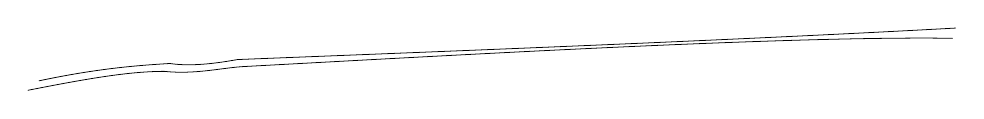
\begin{tikzpicture}[x=1cm,y=1cm,line cap=round]
\draw[line width=.28pt] (0,0) .. controls (.80,.17) and (1.34,.20) .. (1.66,.22)
 .. controls (1.93,.18) and (2.24,.22) .. (2.52,.27)
 .. controls (5.05,.37) and (8.73,.51) .. (11.64,.67);
\draw[line width=.28pt] (-.14,-.12) .. controls (.67,.04) and (1.17,.12) .. (1.59,.12)
 .. controls (1.98,.08) and (2.29,.16) .. (2.58,.18)
 .. controls (5.54,.34) and (9.54,.57) .. (11.60,.54);
\end{tikzpicture}}

\margin{\uline{N.B.} (10) is also written \deleted{\unsure{(11)}}
\[
(10\text{ bis})\qquad
(\ell_0^{\gamma}h_0^{-1})\cdot\rho(\ell_0^{\gamma}h_0^{-1})\cdot\rho^2(\ell_0^{\gamma}h_0^{-1})=1
\]
}

\scanpage{59}
\mspage{318}

\[
(11)\qquad
\left\{
\begin{aligned}
u(\ell_0)&=\operatorname{int}(g_0)(\ell_0^p)\\
u(\ell_1)&=\operatorname{int}\bigl(\underbrace{\sigma_\infty(g_0)}_{\inserted{\unsure{g_1}}}\bigr)(\ell_1^p)\\
u(\ell_\infty)&=\operatorname{int}\bigl(g_0\ell_0^{-\unsure{\gamma|\sigma}}\rho^{-1}(h_0)\bigr)(\ell_\infty^p)
\end{aligned}
\right.,
\]

and one must in all rigor, in addition to conditions (9),(10), require that the two elements $u(\ell_0),u(\ell_1)$ \inserted{given by (11)} \unsure{form} generators of the profinite group $\widehat{\Pi}_{0,3}$.
\margin{(11 bis)}

I am going to calculate the action of $u$ on $\widehat{\mathfrak S}_{0,3}^{+}$, considering this group as generated by the elements
\[
(12)\qquad \ell'_1=\sigma_\infty,\qquad \ell'_\infty=\rho^{-1}
\]
so one simply has to calculate \inserted{$\operatorname{int}(u).\sigma_\infty=u(\sigma_\infty)=$} $u\sigma_\infty u^{-1}$ and $u(\rho)=\operatorname{int}(u).\rho=u\rho u^{-1}$. One has by construction ($u$ \unsure{commuting} with $\sigma_\infty$)
\[
(13)\qquad u\unsure{\circ}\sigma_\infty u^{-1}=\sigma_\infty,
\]
and on the other hand one verifies that
\[
\deleted{u(\rho)=u\rho u^{-1}=\operatorname{int}(h}
\]
\[
(14)\qquad \deleted{u\rho}\quad
\left\{
\begin{aligned}
\rho^{-1}u\rho&=\operatorname{int}(h)u\\
\inserted{\text{with}}\quad h&=(\rho^{-1}\sigma_\infty)(g_0)\ell_0^{\gamma}g_0^{-1}
\end{aligned}
\right.
\]
\margin{i.e. $u\rho u^{-1}=\rho\operatorname{int}(h).$\\
$=\operatorname{int}(\rho(h))\rho$\\
i.e. $\rho(h)=\sigma_\infty(g_0)\ell_1^{\gamma}\rho(g_0)^{-1}$}

so one finds, in \unsure{terms} of an operation on the group $\widehat{\mathfrak S}_{0,3}^{+}$ generated by \inserted{$\ell'_1=$}$\sigma_\infty$ and \inserted{$\ell'_\infty=$}$\rho^{-1}$ (or $\rho$)
\[
(15)\qquad
\left\{
\begin{aligned}
u(\sigma_\infty)&=\sigma_\infty\\
u(\rho)&=g.\rho
\end{aligned}
\right.
\quad\inserted{\text{with}}\quad
 g=\sigma_\infty(g_0)\ell_1^{\unsure{\gamma|\tau}}\rho(g_0)^{-1}
\]

\scanpage{60}

\uline{N.B.} The relation \deleted{$u(\rho)^3=1$} $u(\sigma_\infty)^2=1$ is trivial, the relation $u(\rho)^3=1$ reduces to
\[
\deleted{g\rho(g)\unsure{=}}
\]
\[
(16)\qquad g\rho(g)\rho^2(g)=1
\]
which is a consequence of the explicit expression (15) for $g$, and of formula (10).

Let us note that one \deleted{\unsure{will have}} \inserted{should have}, \& \unsure{taking up again}
\[
\ell'_0=\sigma_\infty\rho=\unsure{\varepsilon_0|e_0}\qquad
(\text{\unsure{whence}}\quad \ell_0^{\prime 2}=\ell_0)
\]
\[
(17)\qquad
u(\unsure{\ell'_0})
=\operatorname{int}(g_0)(\ell_0^{\prime p})
\]
\inserted{\figure{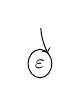
\begin{tikzpicture}[x=1cm,y=1cm,baseline=-0.45ex,line width=0.35pt]
\draw[->] (0.01,0.45) .. controls (0.02,0.31) and (0.06,0.22) .. (0.10,0.13);
\draw (0,0) ellipse [x radius=0.15cm,y radius=0.18cm];
\node[inner sep=0pt] at (0,-0.01) {$\scriptstyle\unsure{\varepsilon}$};
\end{tikzpicture}}}
\margin{?}
--- this relation \unsure{when|when} squared is none other than the first relation (11)
\[
u(\ell_0)=\operatorname{int}(g_0)(\ell_0^p).
\]

[The relation (17) is a consequence of it, if one admits that the centralizer of $L_0=\ell_0^{\widehat{\mathbb Z}}$ in $\widehat{\Pi}_{0,3}$ is reduced to $L_0$\ldots]

One should also have the relation
\[
(18)\qquad u(\rho)\deleted{\unsure{\equiv|=}}\inserted{\text{conjugate of}}\rho^p
\quad\deleted{\text{\unsure{mod|modulo}}\ \widehat{\Pi}_{0,3}}
\]
\deleted{\illegible{1}} to which we \unsure{are going to} return -- it is not clear to me that it is a consequence of the conditions \unsure{considered} on $u$ up to now.
\margin{\deleted{\illegible{2}}}
